\documentclass[spanish,A4,11pt]{article}
\usepackage[left=2cm,top=2cm,right=2cm,bottom=2cm]{geometry} 
\usepackage[utf8]{inputenc}
\usepackage{tikz}
\usepackage{enumitem}
\usepackage{array}
\usepackage[spanish]{babel}
\usepackage{graphicx} 
\usepackage{placeins}
\usepackage{makeidx}
\usepackage{multirow, array}
\usepackage{float}
\usepackage{tabularx}
\usepackage{adjustbox}
\usepackage[vlines]{tabularht}
\usepackage{fancyhdr}
\pagestyle{fancy}
\lhead{DESCRIPCIÓN DEL MERCADO} 
\rhead{Daniel Czarnievicz, Paula Pereda, Joaquín Pereira}
\begin{document}

\section{Agentes}
\noindent \textbf{Composición de la oferta:}  
\begin{itemize}[noitemsep]
\item ANCAP: monopolio importador y refinador de petróleo.
\item Distribuidoras: encargadas de transportar los productos desde ANCAP hacia las estaciones mediante la contratación de empresas de fletes.
\begin{itemize}[noitemsep]
\item DUCSA: distribuye combustible y lubricantes ANCAP y Chevron, es quien percibe el alquiler de las EESS que alquilan la propiedad, dueña de dos EESS, dueña de las franquicias 360. 
\item Petrobras: distribuye combustible, y lubricantes de su marca
\item Axion: distribuye combustible, y lubricantes de su marca
\end{itemize}
\item Las estaciones de servicios (EESS): son las encargadas de realizar la venta al público, son operadas por empresas privadas bajo el sello de la distribuidora correspondiente. Pueden ser dueñas o no de la propiedad en la cual opera la estación. Existen 488 estaciones en el territorio nacional distribuidas según se muestran en el Cuadro 1 y Figura 1 del anexo.
\end{itemize}

Tal como se desprende del informe elaborado por CPA Ferrere para la UNVENU, en términos agregados, la venta de combustibles ha mostrado un patrón similar al del nivel de la actividad económica: mientras el PIB creció a una tasa promedio de 5,6\% entre 2005 y 2013, la venta de combustibles creció 5,0\% en el mismo período. Sin embargo, si se descompone la oferta por tipo de combustible, el patrón es disímil: la venta de gasoil tuvo incrementos moderados, creciendo en promedio menos de la mitad de lo que lo hizo la venta total de combustible (2,1\% en el período 2005-2013). Por su parte, la nafta presentó un crecimiento promedio superior al 10\% en el mismo período. De este modo, la nafta fue la que sustentó el dinamismo del negocio de venta de combustibles, pasando a representar en 2015 casi la mitad de las ventas totales.\newline

\noindent \textbf{Composición de la demanda:}
\begin{itemize}[noitemsep]
\item Familias y hogares.
\item Empresas.
\item Aeropuerto (este ítem no será tratado en nuestro trabajo).
\end{itemize}

La demanda se caracteriza por ser inelástica. Se distinguen dos categorías de demandantes. Por un lado están las familias y los hogares para quienes los combustibles son un bien de consumo. Por otro lado están las empresas, para quienes los combustibles es un insumos. Por lo tanto, se deben estimar dos curvas de demanda distintas.

\section{Mercados conexos}

ANCAP es un conglomerado que participa en varios mercados, incluyendo combustibles, gas, alcoholes, cemento, entre otros. En este trabajo nos enfocaremos en la integración vertical del mercado de producción y distribución de combustibles líquidos. 

\section{Dinámica del mercado de combustibles líquidos}

La cadena comienza cuando ANCAP importa el petróleo crudo. Este es entregado en la boya de Jos Ignacio, y transportado por oleoducto hasta la refinería de La Teja donde es convertido en sus distintos derivados: naftas, querosene, gasoil, lubricantes, entre otros.

Luego de refinado, el combustible es vendido a las distribuidoras: DUCSA, Petrobras, y Axion. DUCSA se encarga de vender al 59.22\% de las EESS, Petrobras se encarga de vender al 18.24\%, y Axion es quien vende al restante 22.54\% de las EESS.

Las distribuidoras contratan empresas privadas de fletes, las cuales se encargan de transportar los productos a las EESS.

El último eslabón de la cadena lo componen las EESS, quienes se encargan de vender el producto al consumidor final (ver Figura 2 en el anexo). 

\section{Regulación}

Dadas las características del mercado existe una fuerte regulación que podría dividirse en dos categorías: por un lado, la regulación que refiere a la operativa y seguridad, y por otro lado, la regulación comercial y económica. En este trabajo nos referiremos a esta última.

Dentro de la regulación comercial y económica, se destacan:
\begin{itemize}[noitemsep]
\item Por la Ley número 8764 con fecha 15/10/1931, artículo 1, inciso b, ANCAP es un monopolio legal multiproducto con el derecho exclusivo a la ``importación y refinación de petróleo crudo y sus derivados en todo el territorio de la República'', este mercado se encuentra bajo una fuerte regulación.
\item El precio intermedio es fijado a través de la paramétrica. Esta es la regla mediante la cual se fija la rentabilidad bruta de la venta de combustibles de las EESS. La paramátrica pretende reflejar la estructura de costos de una estación tipo. La estación tipo se construyó a partir de una muestra de 52 EESS y sus respectivas estructuras de costos. No obstante, la estación tipo no se derivó directamente de la muestra sino luego de negociaciones entre la UNVENU y ANCAP.
\item El precio final máximo es fijado por el Poder Ejecutivo mediante decretos ante solicitud del directorio de ANCAP.
\item Existen amplios subsidios para el gasoil en ciertos sectores.
\item El sector está sujeto a la regulación impositiva vigente en el país (IMESA, IVA, IRAE, etc.).
\end{itemize}

\newpage

\section{Anexo}

\begin{table}[H]
\centering
\textbf{\caption}{Cantidad y porcentaje de EESS, autos y vehículos por estación de servicio por departamento.}    
\resizebox{17.5cm}{!} {
\begin{tabular}{| c | c | c | c | >{\centering\arraybackslash} m{3cm} | >{\centering\arraybackslash} m{3cm} |}
\hline
\hline
\textbf{Departamento} & \textbf{EESS} & \textbf{EESS (\%)} & \textbf{Vehículos} & \textbf{\% del parque automotor}& \textbf{Vehículos por EESS} \\
\hline
\hline
Artigas & 8 & 1.64\% & 488 & 1.39\% & 61.00 \\
\hline
Canelones & 67 & 13.73\% & 5173 & 14.76\% & 77.21 \\
\hline
	Cerro Largo & 10 & 2.05\% & 1244 & 3.55\% & 124.40 \\
	\hline
	Colonia & 42 & 8.61\% & 1607 & 4.59\% & 38.26 \\
	\hline
	Durazno & 12 & 2.46\% & 819 & 2.34\% & 68.25 \\
	\hline
	Flores & 7 & 1.43\% & 308 & 0.88\% & 44.00 \\
	\hline
	Florida & 15 & 3.07\% & 666 & 1.90\% & 44.40 \\
	\hline
	Lavalleja & 12 & 2.46\% & 504 & 1.44\% & 42.00 \\
	\hline
	Maldonado & 28 & 5.74\% & 3535 & 10.09\% & 126.25 \\
	\hline
	Montevideo & 153 & 31.35\% & 12038 & 34.35\% & 78.68 \\
	\hline
	Paysandú & 22 & 4.51\% & 1234 & 3.52\% & 56.09 \\
	\hline
	Río Negro & 13 & 2.66\% & 567 & 1.62\% & 43.62 \\
	\hline
	Rivera & 8 & 1.64\% & 592 & 1.69\% & 74.00 \\
	\hline
	Rocha & 15 & 3.07\% & 774 & 2.21\% & 51.60 \\
	\hline
	Salto & 13 & 2.66\% & 1590 & 4.54\% & 122.31 \\
	\hline
	San José & 23 & 4.71\% & 1350 & 3.85\% & 58.70 \\
	\hline
	Soriano & 19 & 3.89\% & 968 & 2.76\% & 50.95 \\
	\hline
	Tacuarembó & 13 & 2.66\% & 1023 & 2.92\% & 78.69 \\
	\hline
	Treinta y Tres & 8 & 1.64\% & 568 & 1.62\% & 71.00 \\
	\hline
	\textbf{Total} & \textbf{488} & \textbf{100.00\%} & \textbf{35048} & \textbf{100.00\%} & \textbf{-} \\
	\hline
	\end{tabular}%
}
\end{table}
\FloatBarrier
\noindent\textbf{Fuente:} Elaboración propia en base a datos del Sistema Único de Cobro de Ingresos Vehiculares (SUCIVE) y la Unidad Reguladora de Servicios de Energía y Agua (URSEA).\newline

\begin{figure}[H]
\textbf{\caption}{Mapa de ubicación de las estaciones en el territorio nacional según la distribuidora proveedora}
\centering
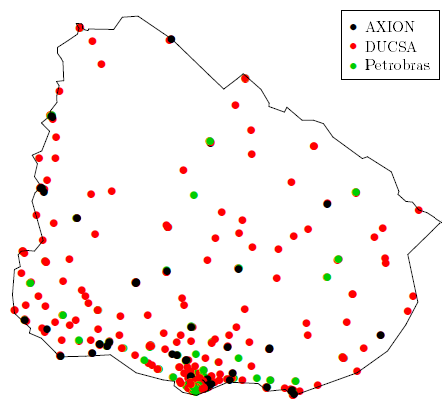
\includegraphics[width=0.8\textwidth]{mapaeess.png}
\end{figure}
\FloatBarrier
\noindent\textbf{Fuente:} Elaboración propia en base a datos de la Unidad Reguladora de Servicios de Energía y Agua (URSEA).\newline

\begin{figure}[H]
\textbf{\caption}{Diagrama de la dinámica de los combustibles líquidos}
\centering
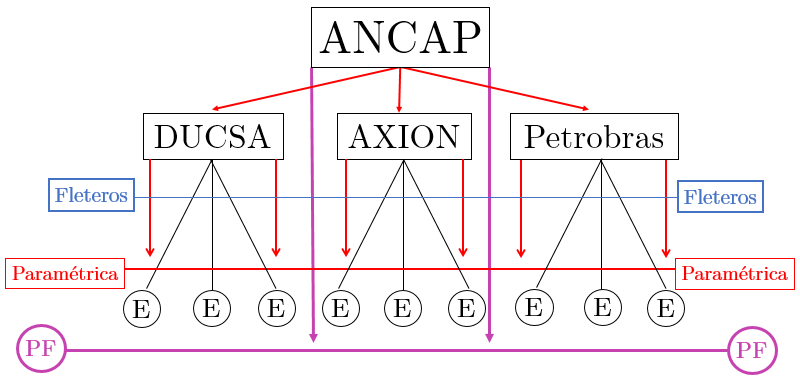
\includegraphics[width=0.8\textwidth]{cadenaeess.png}
\end{figure}

\end{document}
